\documentclass{article}
% generated by Madoko, version 1.1.3
%mdk-data-line={1}


\usepackage[heading-base={2},section-num={False},bib-label={hide},fontspec={True}]{madoko2}


\begin{document}



%mdk-data-line={5}
\mdxtitleblockstart{}
%mdk-data-line={5}
\mdxtitle{\mdline{5}Angel调研及使用报告}%mdk
\mdxauthorstart{}
%mdk-data-line={10}
\mdxauthorname{\mdline{10}ryanyycao(曹洋毓)}%mdk
\mdxauthorend\mdtitleauthorrunning{}{}\mdxtitleblockend%mdk

%mdk-data-line={7}
\section{\mdline{7}1.\hspace*{0.5em}\mdline{7}综述}\label{section}%mdk%mdk

%mdk-data-line={9}
\noindent\mdline{9}\hspace*{1em}\mdline{9}\hspace*{1em}\mdline{9}Angel是一个基于参数服务器的高性能分布式机器学习平台,核心设计理念围绕机器学习模型,将高维度的大模型合理切分到多个参数服务器节点。
Angel的主要核心抽象是PSModel,它将对分布于多台PS Server上的远程模型操作透明化,通过PSModel,用户可以方便的进行模型的更新、
自定义函数计算、同步控制,从而实现各种高效的机器学习算法。Angel基于Java和Scala进行开发,可以使用Yarn直接调度运行,并且支持
Spark on Angel%mdk

%mdk-data-line={14}
\section{\mdline{14}2.\hspace*{0.5em}\mdline{14}架构设计}\label{section}%mdk%mdk

%mdk-data-line={15}
\subsection{\mdline{15}2.1.\hspace*{0.5em}\mdline{15}Angel中的各种角色:}\label{sec-angel}%mdk%mdk

%mdk-data-line={18}
\begin{mddefinitions}%mdk

\mddefterm{\noindent{\bfseries Client}}%mdk

%mdk-data-line={18}
\begin{mdbmarginx}{}{}{}{1.5em}%mdk
\begin{mddefdata}%mdk
\mdline{18}\hspace*{1em}\mdline{18}\hspace*{1em}\mdline{18}控制任务运行,启动和停止Angel任务,加载和存储模型,启动具体计算过程和获取任务运行状态等
%mdk
\end{mddefdata}%mdk
\end{mdbmarginx}%mdk

\mddefterm{\noindent{\bfseries Master}}%mdk

%mdk-data-line={20}
\begin{mdbmarginx}{}{}{}{1.5em}%mdk
\begin{mddefdata}%mdk
\mdline{20}\hspace*{1em}\mdline{20}\hspace*{1em}\mdline{20}原始计算数据以及参数矩阵的分片和分发,申请Worker和ParameterServer所需的计算资源,协调、管理和监控Worker以及ParameterServer
%mdk
\end{mddefdata}%mdk
\end{mdbmarginx}%mdk

\mddefterm{\noindent{\bfseries Parameter Server}}%mdk

%mdk-data-line={22}
\begin{mdbmarginx}{}{}{}{1.5em}%mdk
\begin{mddefdata}%mdk
\mdline{22}\hspace*{1em}\mdline{22}\hspace*{1em}\mdline{22}负责存储和更新参数
%mdk
\end{mddefdata}%mdk
\end{mdbmarginx}%mdk

\mddefterm{\noindent{\bfseries Worker}}%mdk

%mdk-data-line={24}
\begin{mdbmarginx}{}{}{}{1.5em}%mdk
\begin{mddefdata}%mdk
\mdline{24}\hspace*{1em}\mdline{24}\hspace*{1em}\mdline{24}负责具体的模型训练或者结果预测,一个计算任务往往包含许多个Worker实例,每个Worker实例负责使用一部分训练数据进行训练%mdk
\end{mddefdata}%mdk
\end{mdbmarginx}%mdk
%mdk
\end{mddefinitions}%mdk

%mdk-data-line={26}
\noindent\mdline{26}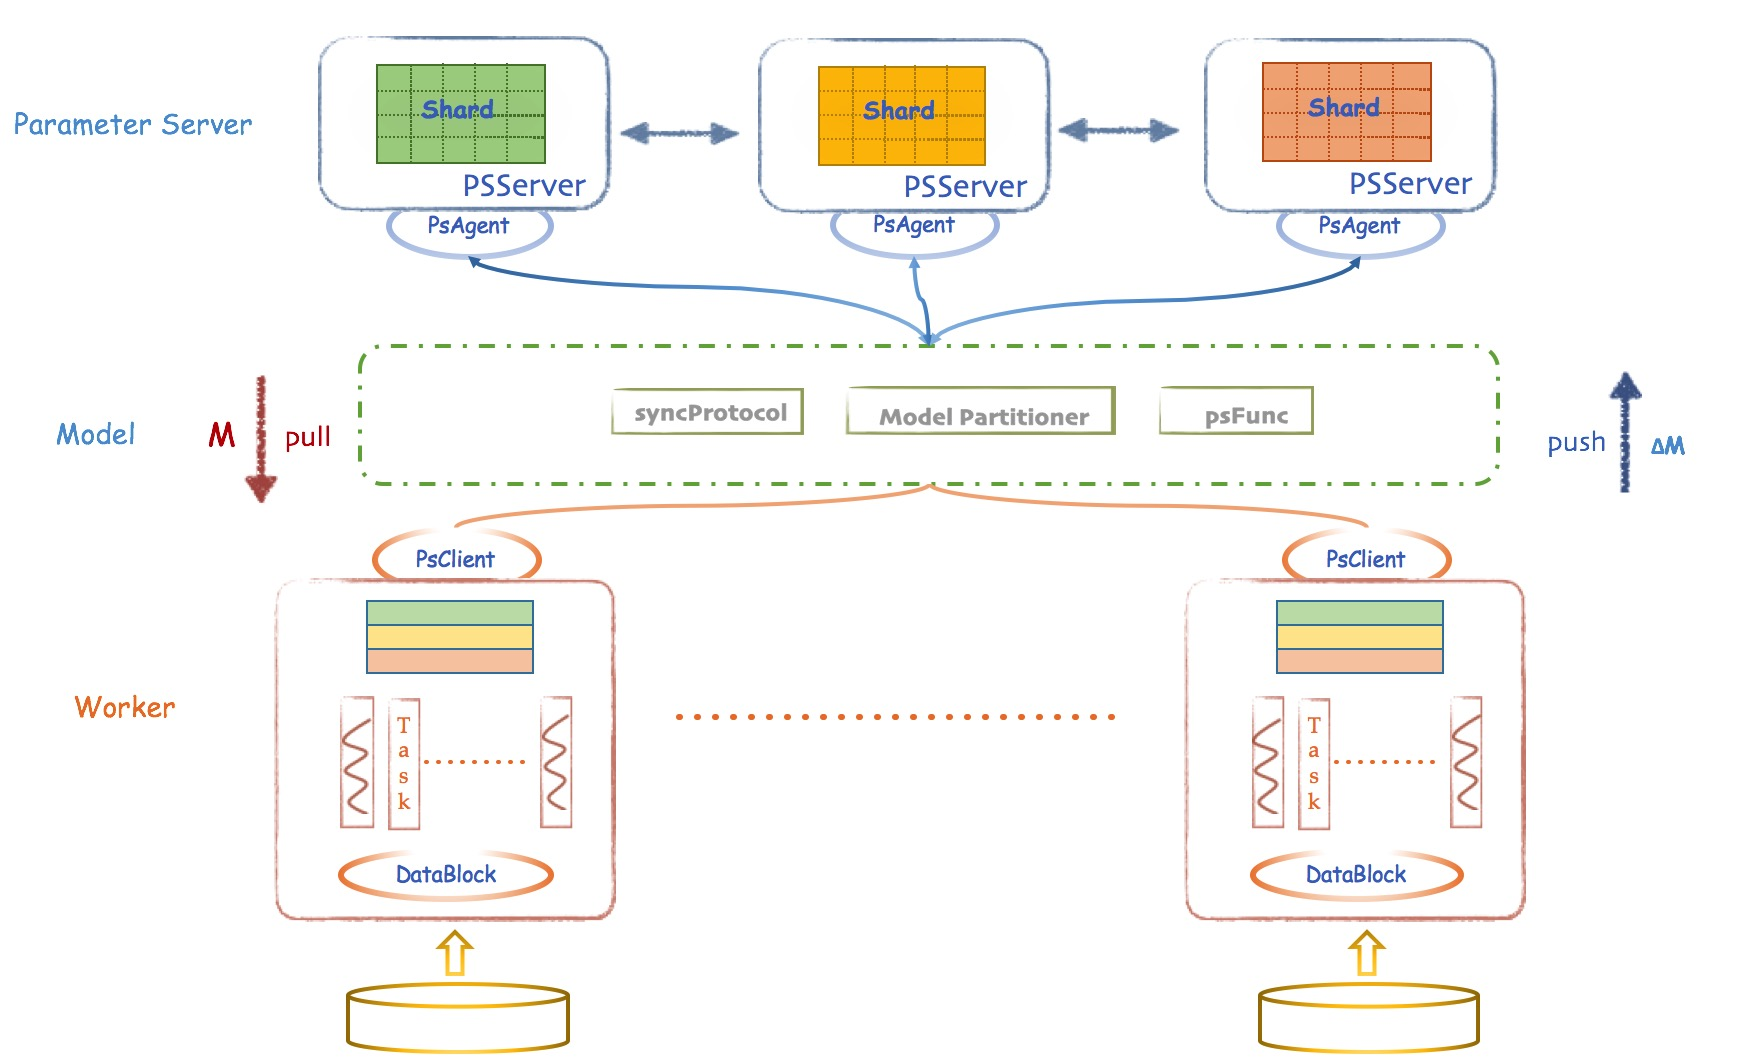
\includegraphics[keepaspectratio=true,width=\dimmin{}{\dimwidth{0.90}}]{images/angel_architecture_1}{}\mdline{26}
\mdline{27} \mdline{27}%mdk

%mdk-data-line={30}
\subsection{\mdline{30}2.2.\hspace*{0.5em}\mdline{30}Angel中的核心抽象:}\label{sec-angel}%mdk%mdk

%mdk-data-line={32}
\begin{mddefinitions}%mdk

\mddefterm{\noindent{\bfseries PSModel}}%mdk

%mdk-data-line={32}
\begin{mdbmarginx}{}{}{}{1.5em}%mdk
\begin{mddefdata}%mdk
\mdline{32}\hspace*{1em}\mdline{32}\hspace*{1em}\mdline{32}PSModel是一个远程模型的概念,对于Client来说,它是一个类似模型代理的类。通过它你可以在每个Worker上,像操作本地对象一样去操作一个模型,而实际上你操作的是一个均匀切分在远程多个PSServer上的分布式模型切片,而且所有的操作都是透明并发的
%mdk
\end{mddefdata}%mdk
\end{mdbmarginx}%mdk

\mddefterm{\noindent{\bfseries MLModel}}%mdk

%mdk-data-line={34}
\begin{mdbmarginx}{}{}{}{1.5em}%mdk
\begin{mddefdata}%mdk
\mdline{34}\hspace*{1em}\mdline{34}\hspace*{1em}\mdline{34}由一系列的PSModel(远程模型)构成,对这些模型进行统一操作%mdk
\end{mddefdata}%mdk
\end{mdbmarginx}%mdk
%mdk
\end{mddefinitions}%mdk

%mdk-data-line={37}
\section{\mdline{37}3.\hspace*{0.5em}\mdline{37}高级特性}\label{section}%mdk%mdk

%mdk-data-line={39}
\subsection{\mdline{39}3.1.\hspace*{0.5em}\mdline{39}多种参数同步协议(通过向量时钟实现)}\label{section}%mdk%mdk

%mdk-data-line={40}
\begin{itemize}[noitemsep,topsep=\mdcompacttopsep]%mdk

%mdk-data-line={40}
\item{}
%mdk-data-line={40}
\mdline{40}BSP:在每一轮迭代中都需要等待所有的Task计算完成%mdk%mdk

%mdk-data-line={42}
\item{}
%mdk-data-line={42}
\mdline{42}SSP:允许一定程度的Task进度不一致,但这个不一致有一个上限%mdk%mdk

%mdk-data-line={44}
\item\mdline{44}ASP:Task之间完全不用相互等待,先完成的Task,继续下一轮的训练%mdk
%mdk
\end{itemize}%mdk

%mdk-data-line={46}
\subsection{\mdline{46}3.2.\hspace*{0.5em}\mdline{46}ps function(psf)}\label{sec-ps-functionpsf}%mdk%mdk

%mdk-data-line={48}
\begin{itemize}%mdk

%mdk-data-line={48}
\item{}
%mdk-data-line={48}
\mdline{48}设计理念%mdk

%mdk-data-line={50}
\mdline{50}\hspace*{1em}\mdline{50}\hspace*{1em}\mdline{50}实际应用中,各个算法对参数服务器上的参数获取和更新,远远不只pull()/push()这么简单,尤其是当算法需要实施一些特定的优化的时候。psf可以支持在ps端做一些简单的计算,从而在计算开销不变的情况下降低通信开销。随着psFunc的引入,模型的计算,也会发生在PSServer端,
PSServer也将有一定的模型计算职责,而不是单纯的模型存储功能。%mdk

%mdk-data-line={53}
\mdline{53}\hspace*{1em}\mdline{53}\hspace*{1em}\mdline{53}我们可以通过继承Angel提供的psf函数接口来设计自己的参数获取更新逻辑,合理的设计psFunc,将大大的加速算法的运行。
伴随着psFunc的引入和强化,在很多复杂的算法实现中,大大的降低了Worker要把模型完整的拖回来进行整体计算的可能性,从而提升算法效率。%mdk%mdk

%mdk-data-line={56}
\item{}
%mdk-data-line={56}
\mdline{56}整体架构%mdk

%mdk-data-line={58}
\mdline{58}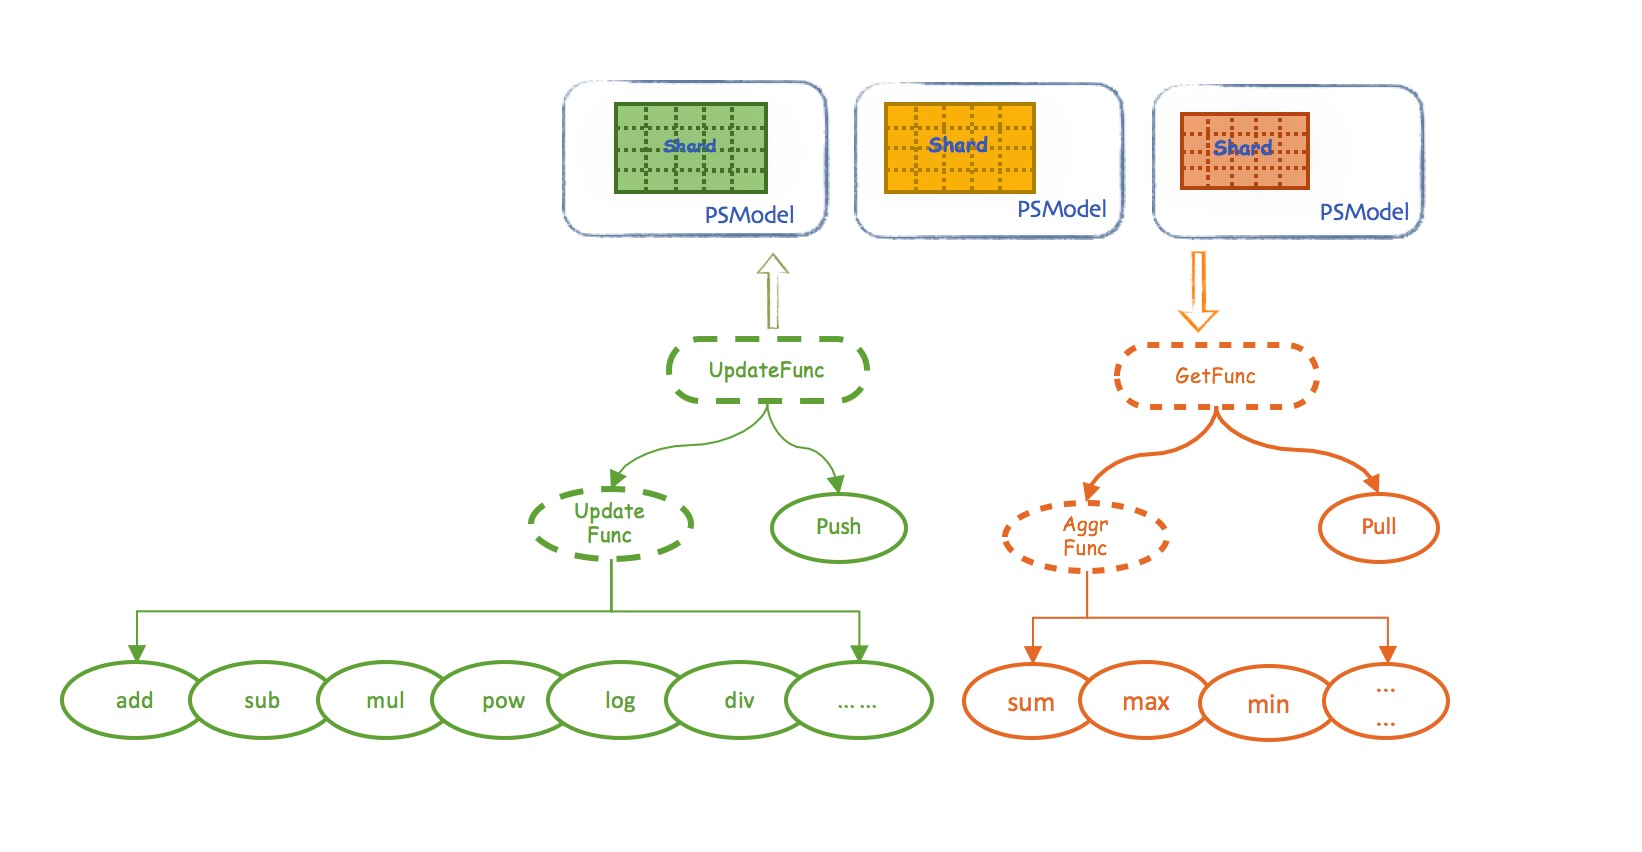
\includegraphics[keepaspectratio=true,width=\dimmin{}{\dimwidth{0.90}}]{images/angel_psFunc}{}\mdline{58}%mdk%mdk

%mdk-data-line={60}
\item{}
%mdk-data-line={60}
\mdline{60}GetFunc(参数获取)%mdk

%mdk-data-line={62}
\mdline{62}请求划分:操作的是整个模型参数,进行请求划分,生成一个请求列表,这个请求列表中,每一个请求都和一个模型参数分区对应%mdk

%mdk-data-line={64}
\mdline{64}请求发送:将请求列表中的所有请求,发送给模型参数分区所在的PSServer,PSServer以模型参数分区为单位执行参数获取和更新操作,并返回相应的结果%mdk

%mdk-data-line={66}
\mdline{66}请求合并:合并所有的模型分区级结果,得到最终的结果并返回%mdk%mdk

%mdk-data-line={68}
\item{}
%mdk-data-line={68}
\mdline{68}UpdateFunc(参数更新)%mdk

%mdk-data-line={70}
\mdline{70}请求划分:PSClient进行请求划分,生成一个请求列表,这个请求列表中的每一个请求都和一个模型参数分区对应%mdk

%mdk-data-line={72}
\mdline{72}请求发送:将请求列表中的所有请求发送给模型参数分区所在的PS实例,PS实例以模型参数分区为单位执行更新操作%mdk

%mdk-data-line={74}
\mdline{74}等待完成:等待所有请求完成后返回%mdk

%mdk-data-line={76}
%mdk-data-line={77}
\noindent\mdline{77}\textbf{Note}.
\mdline{78}无论是Get还是Update,具体的这三个阶段,其过程都是可以自定义的,从而实现千变万化的psFunc。%mdk%mdk

%mdk-data-line={79}
%mdk-data-line={80}
\noindent\mdline{80}\textbf{Note}.
\mdline{81}之前github相关文档中提到psf分为client-ps的psf和ps-ps的psf,后联系作者确认并没有ps-ps的psf,github文档有误。%mdk%mdk%mdk
%mdk
\end{itemize}%mdk

%mdk-data-line={87}
\subsection{\mdline{87}3.3.\hspace*{0.5em}\mdline{87}自定义模型切片}\label{section}%mdk%mdk

%mdk-data-line={89}
\begin{itemize}[noitemsep,topsep=\mdcompacttopsep]%mdk

%mdk-data-line={89}
\item\mdline{89}Angel默认的模型分区:将模型切分成大小相等的矩形区域。1)尽量将一个模型平均分配到所有PS节点上;2)对于非常小的模型,将它们尽量放在一个PS节点上;3)对于多行的模型,尽量将同一行放在一个PS节点上%mdk

%mdk-data-line={90}
\item\mdline{90}自定义模型分区:可以将模型横切或者模型纵切,也支持横切纵切都存在的更复杂的切片方式。设置自定义的Partitioner,实现两个接口getPartitions和assignPartToServer,最后将其将其注入到PSModel的MatrixContext之中即可使用%mdk
%mdk
\end{itemize}%mdk

%mdk-data-line={92}
\subsection{\mdline{92}3.4.\hspace*{0.5em}\mdline{92}支持多种容错}\label{section}%mdk%mdk

%mdk-data-line={93}
\begin{itemize}[noitemsep,topsep=\mdcompacttopsep]%mdk

%mdk-data-line={93}
\item\mdline{93}PS容错采用了checkpoint的模式%mdk

%mdk-data-line={94}
\item\mdline{94}挂掉的Worker实例可以从Master处获取当前迭代轮数等状态信息,从PS处获取最新模型参数,然后重新开始被断掉的迭代%mdk

%mdk-data-line={95}
\item\mdline{95}Master定期将任务状态写入hdfs,挂掉后Yarn会重新拉起一个Angel的Master,加载状态信息,重新启动Worker和PS,从断点处重新开始计算。%mdk
%mdk
\end{itemize}%mdk

%mdk-data-line={97}
\section{\mdline{97}4.\hspace*{0.5em}\mdline{97}Angel编译和运行}\label{sec-angel}%mdk%mdk

%mdk-data-line={99}
\begin{itemize}[noitemsep,topsep=\mdcompacttopsep]%mdk

%mdk-data-line={99}
\item\mdline{99}环境要求:Jdk \mdline{99}\textgreater{}\mdline{99}= 1.8 Maven \mdline{99}\textgreater{}\mdline{99}= 3.0.5 Protobuf \mdline{99}\textgreater{}\mdline{99}= 2.5.0且和Hadoop的Protobuf版本一致%mdk

%mdk-data-line={100}
\item\mdline{100}源码下载:git clone https://github.com/Tencent/angel%mdk

%mdk-data-line={101}
\item\mdline{101}编译:mvn clean package\mdline{101} \mdline{101}-Dmaven.test.skip=true  发布包位于dist/target目录下%mdk

%mdk-data-line={102}
\item\mdline{102}运行时可以选择本地运行,或通过Yarn提交到集群运行

%mdk-data-line={103}
%mdk-data-line={104}
\noindent\mdline{104}\textbf{Note}.
\mdline{105}由于Angel编译要求和Hadoop的Protobuf版本一致,中心集群Hadoop的Protobuf版本为2.4,
而Angel使用Protobuf2.4会报很多方法没有实现的错误,需要修改很多底层源码,暂时来看在中心集群搭建分布式Angel不可行%mdk%mdk%mdk
%mdk
\end{itemize}%mdk

%mdk-data-line={108}
\section{\mdline{108}5.\hspace*{0.5em}\mdline{108}实现新算法流程}\label{section}%mdk%mdk

%mdk-data-line={110}
\begin{enumerate}[noitemsep,topsep=\mdcompacttopsep]%mdk

%mdk-data-line={110}
\item\mdline{110}定义一个模型,继承MLModel,里面定义参数模型及其他的一些配置%mdk

%mdk-data-line={111}
\item\mdline{111}定义一个Task,继承自TrainTask,定义模型的训练过程,需要实现parse()和train()两个方法,分别为解析数据和训练%mdk

%mdk-data-line={112}
\item\mdline{112}定义一个Runner,继承自MLRunner,用于将任务提交到集群,实现train()和predict()两个方法%mdk

%mdk-data-line={113}
\item\mdline{113}对于需要复杂的模型切片和复杂的psf的算法,需要自定义模型切片方式和psf

%mdk-data-line={114}
%mdk-data-line={115}
\noindent\mdline{115}\textbf{Note}.
\mdline{116}之前准备基于Angel开发的Distributed Negative Sampling for Word Embeddings算法强依赖于ps-ps的psf,
现在发现Angel并不支持这种ps到ps通信的特性,基于Angel只能实现简单的Word2Vec算法,暂时放弃这个方案%mdk%mdk%mdk
%mdk
\end{enumerate}%mdk

%mdk-data-line={119}
\section{\mdline{119}6.\hspace*{0.5em}\mdline{119}总结}\label{section}%mdk%mdk

%mdk-data-line={120}
\noindent\mdline{120}\hspace*{1em}\mdline{120}\hspace*{1em}\mdline{120}通过这次基于Angel的实践,大概摸索到了Angel的能力范围。Angel核心抽象为模型,特色为将模型分布于多台PS Server,然后提供一整套的psf来对远程模型进行操作。
在支持了自定义模型分区策略、自定义client-ps的psf的高级特性之后,它的优势就很明显的体现了出来。%mdk

%mdk-data-line={123}
\mdline{123}\hspace*{1em}\mdline{123}\hspace*{1em}\mdline{123}对于基于ps的算法来说,这两个特性可以很好的安排模型的分布,安排计算的位置(client or ps),降低通信量,可以明显的提升某些机器学习算法的性能(类似于之前实现的那种Word2Vec算法)。%mdk

%mdk-data-line={125}
\mdline{125}\hspace*{1em}\mdline{125}\hspace*{1em}\mdline{125}但是对于没有ps概念的算法来说,所有的节点之间需要进行通信,由于Angel不提供ps-ps的psf,因此没有办法完成ps间的交互,因此开发这类算法比较困难(类似于Distributed Negative Sampling for Word Embeddings算法)。%mdk%mdk


\end{document}
